\documentclass[tikz,border=20pt]{standalone}
\usepackage{amsmath,amssymb}
\usepackage{tikz}
\usetikzlibrary{arrows.meta,calc}

\begin{document}
	
	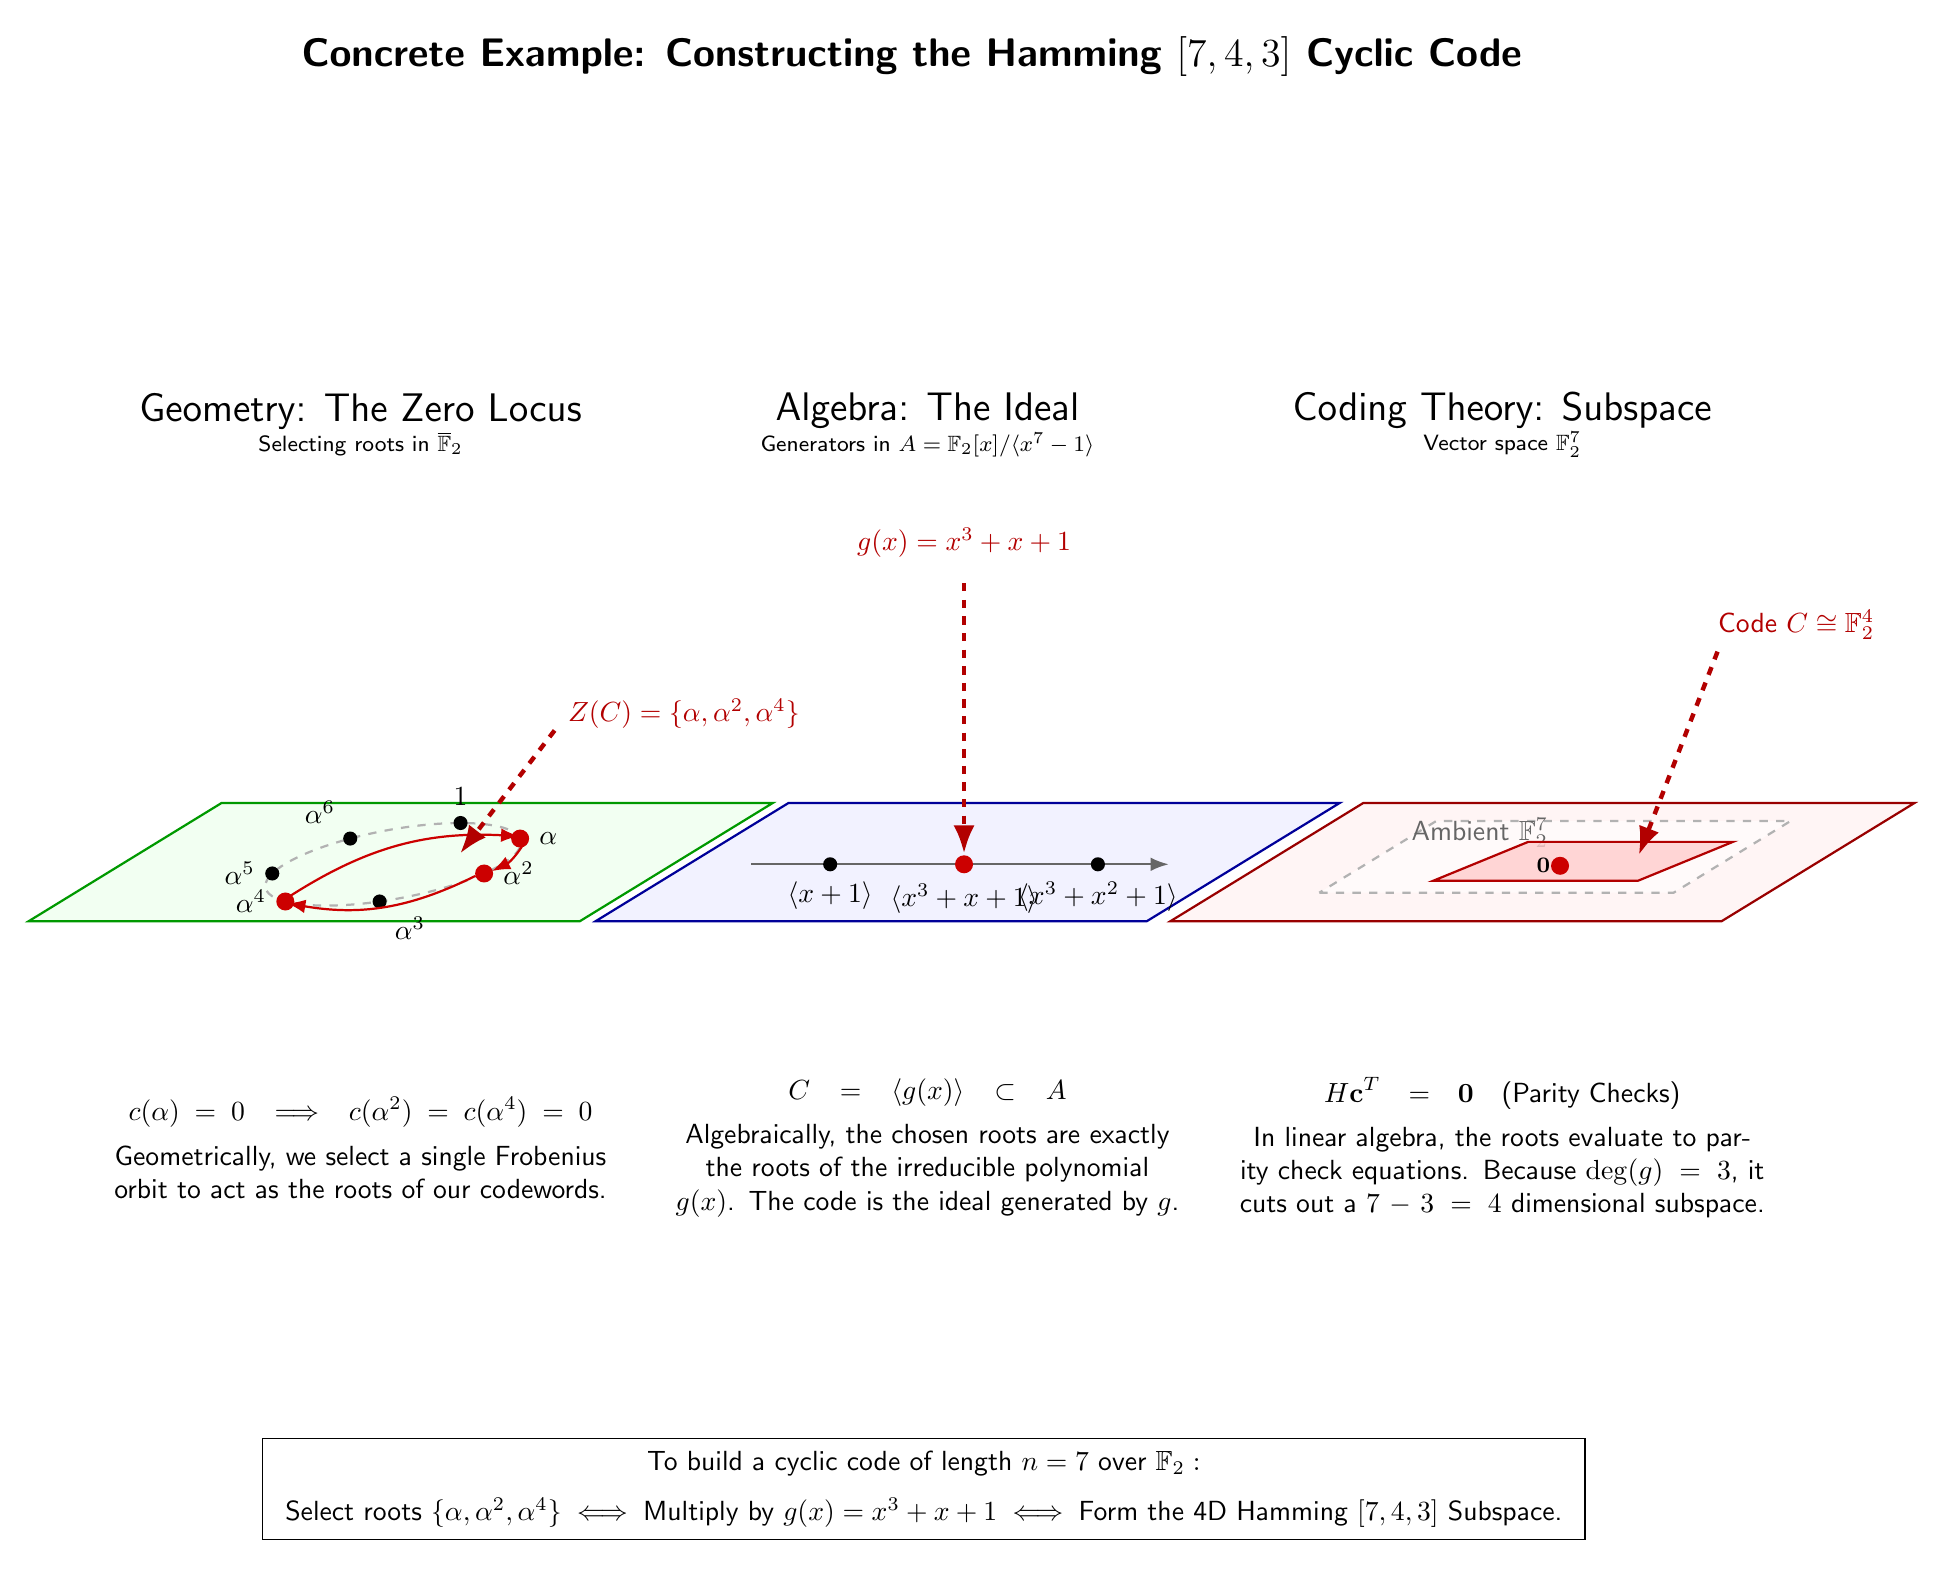
\begin{tikzpicture}[
		x={(1cm,0cm)},
		y={(0.62cm,0.38cm)},
		z={(0cm,1.7cm)},
		scale=1.0,
		font=\sffamily,
		>=Latex,
		pt/.style={circle, fill=black, inner sep=1.8pt},
		sel/.style={circle, fill=red!80!black, inner sep=2.3pt},
		orbA/.style={circle, fill=blue!75!black, inner sep=2.0pt},
		orbB/.style={circle, fill=green!60!black, inner sep=2.0pt}
		]
		
		% =========================================================
		% Global title
		% =========================================================
		\node[align=center] at (0,0,6.2)
		{\Large\bfseries Concrete Example: Constructing the Hamming $[7,4,3]$ Cyclic Code};
		
		% =========================================================
		% LEFT: Geometry (Roots / Zeros of the Code)
		% =========================================================
		\begin{scope}[shift={(-7.2,0,0)}]
			
			\draw[fill=green!5, draw=green!60!black, thick]
			(-3.3,-1.15,0) -- (3.7,-1.15,0) -- (3.7,2.8,0) -- (-3.3,2.8,0) -- cycle;
			
			\node[align=center] at (0.2,0,3.45)
			{\Large Geometry: The Zero Locus\\[-1pt]\footnotesize Selecting roots in $\overline{\mathbb F}_2$};
			
			\coordinate (O) at (0.15,0.75,0);
			\draw[thick, dashed, gray!60] (O) circle (1.38);
			
			\coordinate (P0) at ($(O)+(90:1.38)$);
			\coordinate (P1) at ($(O)+(38.571:1.38)$);
			\coordinate (P2) at ($(O)+(-12.857:1.38)$);
			\coordinate (P3) at ($(O)+(-64.286:1.38)$);
			\coordinate (P4) at ($(O)+(-115.714:1.38)$);
			\coordinate (P5) at ($(O)+(-167.143:1.38)$);
			\coordinate (P6) at ($(O)+(141.429:1.38)$);
			
			% Roots
			\node[pt, label=above:{$1$}] at (P0) {};
			% The selected orbit (Zeros of our code)
			\node[sel, label=right:{$\alpha$}] at (P1) {};
			\node[sel, label=right:{$\alpha^2$}] at (P2) {};
			\node[sel, label=left:{$\alpha^4$}] at (P4) {};
			% The unselected orbit
			\node[pt, label=below right:{$\alpha^3$}] at (P3) {};
			\node[pt, label=left:{$\alpha^5$}] at (P5) {};
			\node[pt, label=above left:{$\alpha^6$}] at (P6) {};
			
			% Conjugacy arrows for the chosen roots
			\draw[->, thick, red!80!black] ($(P1)+(0.05,0.08)$) to[bend left=18] ($(P2)+(0.05,0.08)$);
			\draw[->, thick, red!80!black] ($(P2)+(-0.06,-0.08)$) to[bend left=18] ($(P4)+(0.06,-0.06)$);
			\draw[->, thick, red!80!black] ($(P4)+(-0.05,0.08)$) to[bend left=18] ($(P1)+(-0.06,0.08)$);
			
			\draw[->, ultra thick, dashed, red!70!black] (2.2,0.75,1.0) -- (1.0,0.75,0.08);
			
			\node[align=left, text=red!70!black] at (3.5,1.3,1.0)
			{$Z(C) = \{\alpha, \alpha^2, \alpha^4\}$};
			
			\node[align=center, text width=7.2cm] at (0.2,0,-1.95)
			{$\displaystyle c(\alpha) = 0 \implies c(\alpha^2)=c(\alpha^4)=0$\\[4pt]
				Geometrically, we select a single Frobenius orbit to act as the roots of our codewords.};
			
		\end{scope}
		
		% =========================================================
		% MIDDLE: Algebra (Ideals / Generator Polynomial)
		% =========================================================
		\begin{scope}[shift={(0,0,0)}]
			
			\draw[fill=blue!5, draw=blue!60!black, thick]
			(-3.3,-1.15,0) -- (3.7,-1.15,0) -- (3.7,2.8,0) -- (-3.3,2.8,0) -- cycle;
			
			\node[align=center] at (0.2,0,3.45)
			{\Large Algebra: The Ideal\\[-1pt]\footnotesize Generators in $A = \mathbb F_2[x]/\langle x^7-1\rangle$};
			
			\draw[->, thick, gray!80!black] (-2.5, 0.75, 0) -- (2.8, 0.75, 0);
			
			\node[pt,  label=below:{$\langle x+1\rangle$}] at (-1.5, 0.75, 0) {};
			\node[sel, label=below:{$\langle x^3+x+1\rangle$}] at (0.2, 0.75, 0) {};
			\node[pt,  label=below:{$\langle x^3+x^2+1\rangle$}] at (1.9, 0.75, 0) {};
			
			\draw[->, ultra thick, dashed, red!70!black]
			(0.2,0.75,2.1) -- (0.2,0.75,0.08);
			
			\node[align=center, text=red!70!black] at (0.2,0.75,2.4)
			{$g(x) = x^3+x+1$};
			
			\node[align=center, text width=7.6cm] at (0.2,0,-1.95)
			{$\displaystyle C = \langle g(x) \rangle \subset A$\\[4pt]
				Algebraically, the chosen roots are exactly the roots of the irreducible polynomial $g(x)$. The code is the ideal generated by $g$.};
			
		\end{scope}
		
		% =========================================================
		% RIGHT: Coding Theory (Vector Subspace)
		% =========================================================
		\begin{scope}[shift={(7.3,0,0)}]
			
			\draw[fill=red!4, draw=red!60!black, thick]
			(-3.3,-1.15,0) -- (3.7,-1.15,0) -- (3.7,2.8,0) -- (-3.3,2.8,0) -- cycle;
			
			\node[align=center] at (0.2,0,3.45)
			{\Large Coding Theory: Subspace\\[-1pt]\footnotesize Vector space $\mathbb F_2^7$};
			
			% Ambient Space F_2^7 Grid/Box
			\draw[thick, dashed, gray!60, fill=white, fill opacity=0.5] 
			(-2.0, -0.2, 0) -- (2.5, -0.2, 0) -- (2.5, 2.2, 0) -- (-2.0, 2.2, 0) -- cycle;
			\node[gray!80!black] at (-1.2, 1.8, 0) {Ambient $\mathbb F_2^7$};
			
			% Subspace C
			\draw[thick, fill=red!20, draw=red!70!black, fill opacity=0.8] 
			(-0.8, 0.2, 0) -- (1.8, 0.2, 0) -- (2.2, 1.5, 0) -- (-0.4, 1.5, 0) -- cycle;
			
			\node[sel] (origin) at (0.5, 0.7, 0) {};
			\node[left, font=\footnotesize] at (origin) {$\mathbf{0}$};
			
			\draw[->, ultra thick, dashed, red!70!black]
			(2.5, 0.7, 1.6) -- (1.5, 0.7, 0.08);
			
			\node[align=left, text=red!70!black] at (3.5, 0.7, 1.8)
			{Code $C \cong \mathbb F_2^4$};
			
			\node[align=center, text width=8.2cm] at (0.2,0,-1.95)
			{$\displaystyle H \mathbf{c}^T = \mathbf{0} \quad \text{(Parity Checks)}$\\[4pt]
				In linear algebra, the roots evaluate to parity check equations. Because $\deg(g)=3$, it cuts out a $7-3 = 4$ dimensional subspace.};
			
		\end{scope}
		
		% =========================================================
		% Bottom summary
		% =========================================================
		\node[align=center, text width=16.5cm] at (0,0,-4.5)
		{$\boxed{
				\begin{array}{c}
					\text{To build a cyclic code of length } n=7 \text{ over } \mathbb F_2 : \\[6pt]
					\text{Select roots } \{\alpha, \alpha^2, \alpha^4\}
					\iff
					\text{Multiply by } g(x) = x^3+x+1
					\iff
					\text{Form the 4D Hamming } [7,4,3] \text{ Subspace.}
				\end{array}
			}$};
		
	\end{tikzpicture}
	
\end{document}